\section{Data Preparation}

In order to describe the customers behavior, we extract the following new features from the dataset:
\begin{itemize}
\item the total number of items purchased by a customer;
\item the number of distinct items bought by a customer;
\item the maximum number of items purchased by a customer during a shopping session.
\end{itemize}

In Figure \ref{fig:qta_features}, we can see some visualization for these features; in particular, they represent the first 30 customers with the biggest values for each feature.\\
An interesting information is clear from the plot \ref{fig:max_item}, where we can see that the maximum quantities purchased in a single shopping session are very big; they are all above 3500, with the maximum equal to 15049. These are very high values, unlikely for a retail customer; this led us to think that the supermarket in question also sells wholesale.

\begin{figure}[h!]
\captionsetup{justification=centering}
\begin{subfigure}{.3\textwidth}
\centering
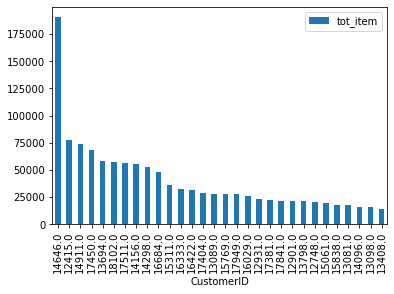
\includegraphics[width=\textwidth]{img/preparation/tot_item.png}
\caption{Total number of items per customer}
\label{fig:tot_item}
\end{subfigure}
\begin{subfigure}{.3\textwidth}
\centering
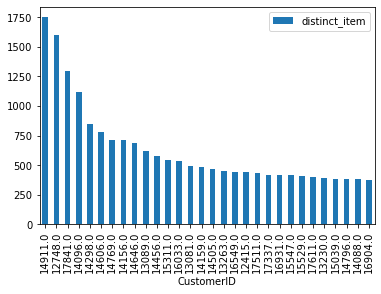
\includegraphics[width=\textwidth]{img/preparation/distinct_item.png}
\caption{Number of distinct items per customer}
\label{ref:distinct_item}
\end{subfigure}
\begin{subfigure}{.3\textwidth}
\centering
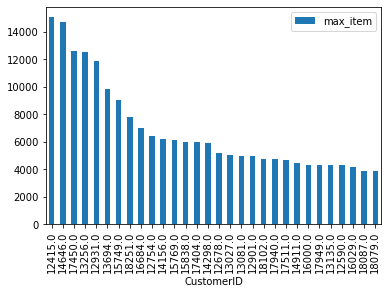
\includegraphics[width=\textwidth]{img/preparation/max_item.png}
\caption{Maximum number of items per customer}
\label{fig:max_item}
\end{subfigure}
\caption{Visualization for the extracted features}
\label{fig:qta_features}
\end{figure}

Now, with respect to the \emph{TotSale} attribute we can take into account:
\begin{itemize}
\item the average price spent by a customer during a shopping session;
\item the Shannon entropy on the purchasing behavior of the customer.
\end{itemize}

The entropy represents the variability of the customer's spending habits; i.e. a bigger value means that the customer did not have a regular behavior since he spent always a different amount of money, while lower values identify predictable spending behavior since the customer tends to spend always the same amount of money.\\
As shown in \ref{fig:features_pairplot}, we have a small peak corresponding to 0, meaning that there are some customers with very specific habits, but the maximum is reached for $\sim 4$, which means that the majority of the clients have a quite unpredictable behavior.

At this point we decide to introduce a domain specific model, called \emph{RFM}, to provide an intresting customer segmentation based on the purchasing behavior of the customers. In particular, the \emph{RFM (Recency, Frequency, Monetary)} analysis refers to:

\begin{itemize}
\item \emph{Frequency} is the number of orders for each customer;
\item \emph{Recency} is the number of days between present date and date of last purchase each customer;
\item \emph{Monetary} is the purchase price for each customer.
\end{itemize}

and it helps divide customers into various categories or clusters to identify customers who are more likely to respond to promotions and also for future personalization services as shown in \ref{fig:features_pairplot}.

\begin{figure}[!h]
\centering
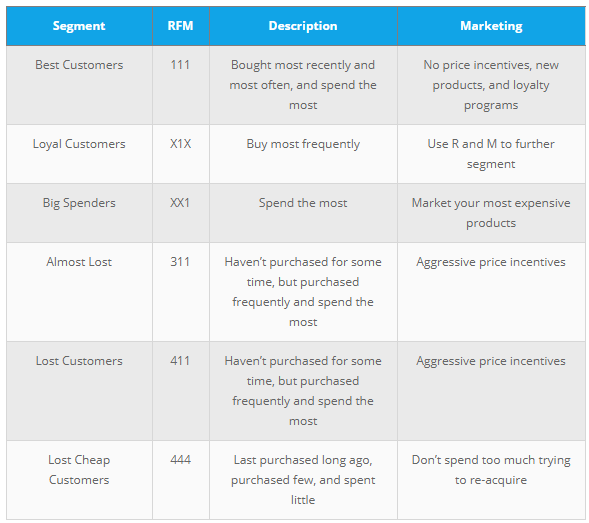
\includegraphics[width=0.5\textwidth]{img/preparation/rfm_seg.png}
\caption{RFM Segmentation}
\label{fig:rfm_seg}
\end{figure}

To calculate the individual RFM we will use the quartil statistical method, i.e. dividing score into four parts, by associating them a number from 1 to 4, so we will deal with the following:

\begin{itemize}
\item best Recency score = 1: most recently purchase
\item best Frequency score = 1: most quantity purchase
\item best Monetary score = 1: spent the most
\end{itemize}

Wrt our dataset the customer segmentation result as following:

\begin{itemize}
\item the number of Best Customers is 394
\item the number of Loyal Customers is 1041
\item the number of Big Spenders is 1052
\item the number of Almost Lost is 112
\item the number of Lost Customers is 28
\item the number of Lost Cheap Customers is 360
\end{itemize}

Now, we can visualize the correlation between the attributes. In Figure \ref{fig:features_corr}, as expected, we find that the average basket value is highly correlated with the total quantity purchased and the amount of money spent. Furthermore, we can see that also the year frequency is correlated with the amount spent and the total quantity. In the end, of course, the quantity purchased is very highly correlated with the total amount spent. Since the dataset deal with both reatil customers and wholesalers we have that some atrtibutes have really spread values. To weight  less the difference between high value with respect the difference between small values we took the logarithm in base ten of those attributes. In Figure \ref{fig:features_corr_logs} and Figure \ref{fig:features_pairplot_logs} we can see the the correlation matrix after computing the logarithm in base ten of \emph{I}, \emph{Iu}, \emph{Imax}, \emph{Savg}, \emph{F} and \emph{M}.

In Figure \ref{fig:pplots}, we can visualize the pairplot for the attributes we have.\\
On the diagonal, we have the density plots, where we can appreciate the distribution of the features. Instead, the other scatter plots show the relationship between two variables. By analyzing those, we can have a confirmation of what we already found thanks to the previous plot. 

\begin{figure}
\begin{subfigure}{.49\textwidth}
\centering
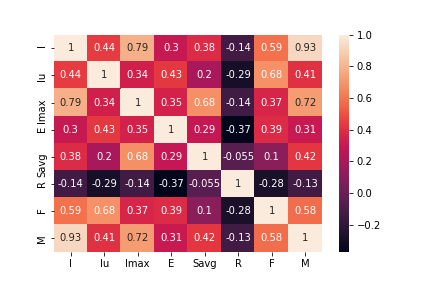
\includegraphics[width=.95\textwidth]{img/preparation/features_corr.png}
\caption{Correlation between the attributes}
\label{fig:features_corr}
\end{subfigure}
\begin{subfigure}{.49\textwidth}
\centering
\captionsetup{justification=centering}
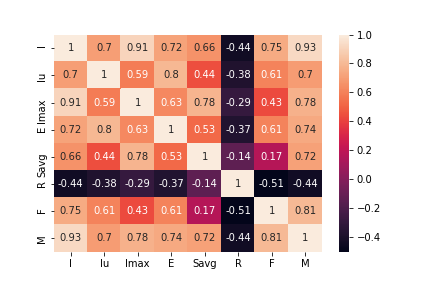
\includegraphics[width=.95\textwidth]{img/preparation/features_corr_logs.png}
\caption{}
\label{fig:features_corr_logs}
\end{subfigure}
\caption{Correlation Matrix before and after log-normalization}
\end{figure}

\begin{figure}
\begin{subfigure}{.49\textwidth}
\centering
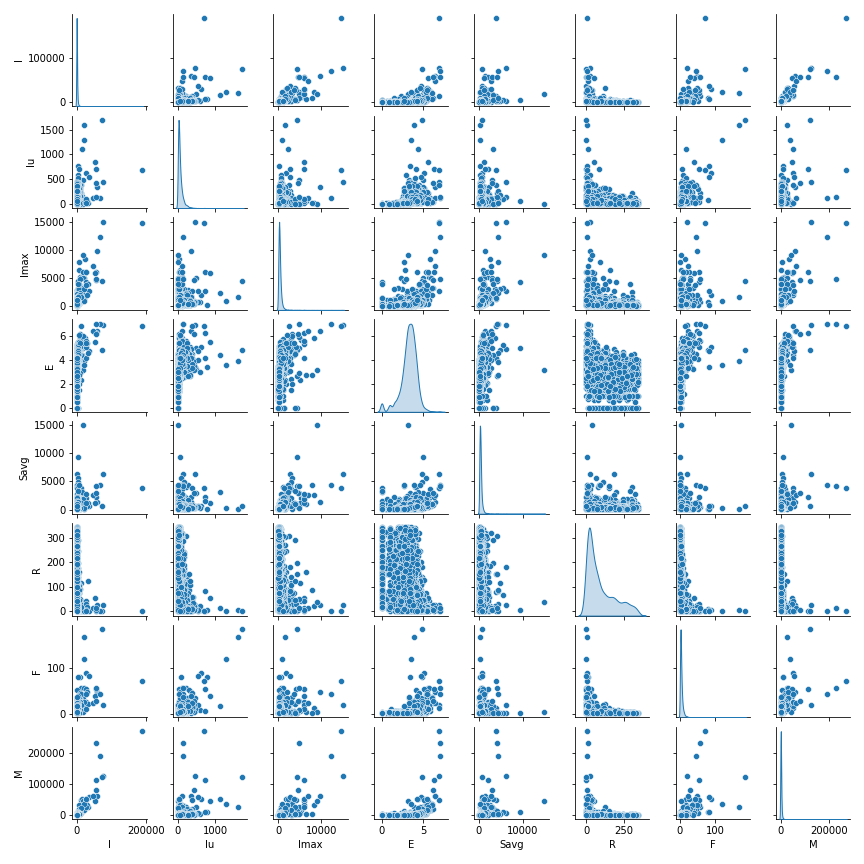
\includegraphics[width=.95\textwidth]{img/preparation/features_pairplot.png}
\caption{}
\label{fig:features_pairplot}
\end{subfigure}
\begin{subfigure}{.49\textwidth}
\centering
\captionsetup{justification=centering}
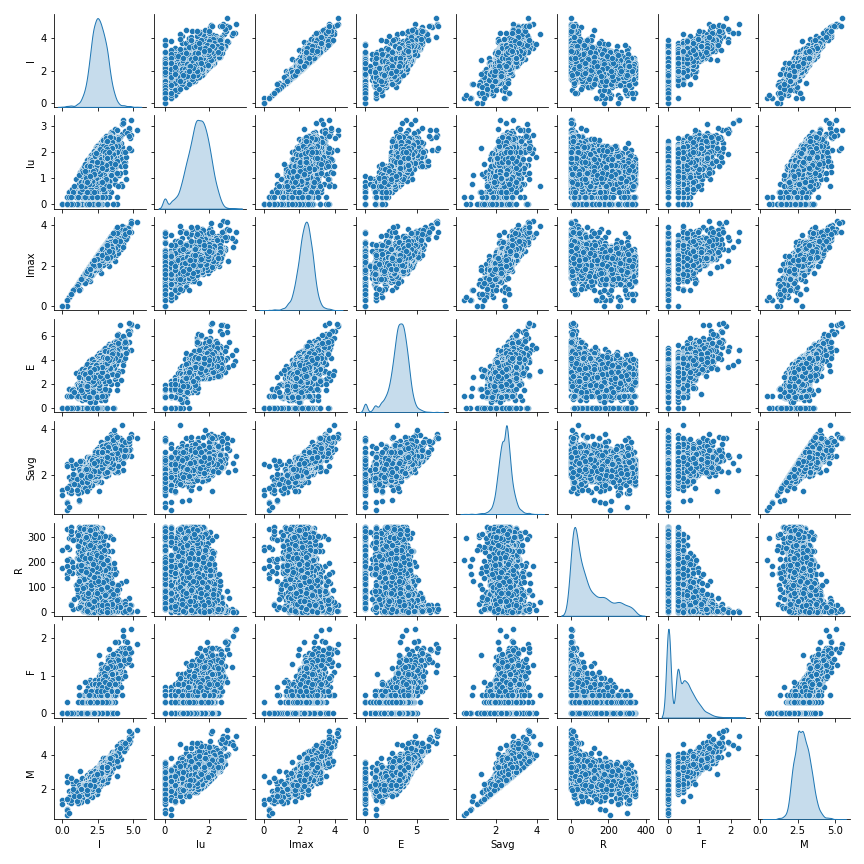
\includegraphics[width=.95\textwidth]{img/preparation/features_pairplot_logs.png}
\caption{}
\label{fig:features_pairplot_logs}
\end{subfigure}
\caption{Pairplots before and after log-normalization}
\label{fig:pplots}
\end{figure}